\section{Caso parallelo a memoria distribuita}
Queste architetture possono essere visualizzate come un grafo in cui i nodi sono processori e gli archi del grafo rappresentano le connessioni dirette.

\uline{Sono processori che non condividono una memoria ma una rete di inter-connessione}, collegati da dei \uline{link full-duplex}\footnote{La comunicazione è simmetrica, può avvenire da entrambi i lati} e possono comunicare tra di loro attraverso questi. 

\paragraph{Proprietà}
In questa architettura i processori sono sincroni ma non hanno una memoria condivisa, c'è una rete di inter-connessione che li lega. In genere, una rete di inter-connessione non mi da un grafo completo. Un grafo dove i nodi sono i processori e gli archi sono i collegamenti diretti tra i processori. I processori hanno una memoria privata per poter lavorare ma manca la memoria centrale condivisa. \uline{Questi processori però condividono un unico clock centrale}. E' un modello di calcolo che da un'astrazione di com'è fatto un super-computer. \uline{Da non confondere con le architetture distribuite, dove non c'è un unico clock centrale e la rete di inter-connessione è Internet}.

Si chiamano distribuiti proprio perchè manca la memoria condivisa.

\paragraph{Caratteristiche dei processori}
Sono sempre delle RAM sequenziali. Sono elementi di calcolo e anche router perchè possono spedire e ricevere informazioni all'interno della rete, \uline{eseguono istruzioni per il calcolo con la loro memoria privata ma devono anche spedire informazioni}. Questo avviene tramite due istruzioni per la comunicazione: \textit{send, receive}.

\paragraph{Proprietà sulla comunicazione} La comunicazione avviene attraverso la spedizione in questa rete, tramite dei messaggi. Rispetto al caso delle P-RAM la comunicazione non è più costante ma dipende dalla distanza tra i processori. La comunicazione è diretta nel momento in cui tra i due processori c'è un link. Tra due processori collegati direttamente il tempo è costante e costa $2$ passi

\paragraph{Cambia Input/Output} 
Manca la memoria condivisa perciò:
\begin{itemize}
    \item Input distribuita tra i processi. Ogni processore avrà qualche dato dell'input
    \item Output o abbiamo un processore dedicato\footnote{Ad esempio il processore con indice più alto ha il risultato} o si legge in un certo ordine tra i vari processori rispettando l'indice dei processori.
\end{itemize}

\paragraph{Risorse di calcolo} Sono sempre tempo e hardware, ma il tempo oltre a contare le operazioni elementari aritmetiche e logiche, conta anche le operazioni di scambio di informazioni (è legato alla rete di connesione e può essere rilevante).

\paragraph{Parametri di rete}
Data un architettura $G=(V,E)$ si definiscono i parametri
\begin{itemize}
    \item GRADO\\
    $$\gamma = max\;\{\;\rho(\upsilon) \;|\; \upsilon \in V \}$$
    \uline{Massimo numero di archi incidenti su un nodo}. Più il grado è alto più ci sono archi, più la connessione può essere buona. Ma se alziamo troppo $\gamma$ per avere migliore comunicazione più difficile diventa la realizzazione fisica
    \item DIAMETRO\\
    $$\delta = max\;\{\;d(\upsilon, \omega)\;|\;\upsilon \neq \omega \in V\;\}$$
    Per ogni coppia di vertici viene definita la distanza tra questi come la minima distanza per raggiungere il nodo destinazione partendo dal nodo iniziale. Questa è rappresentata da $d(\upsilon, \omega)$. \uline{Il diametro è la massima distanza tra due nodi nel grafo}. Valori bassi di $\delta$ sono da preferire nei nostri algoritmi, valori di $\delta$ troppo bassi aumentano il valore di $\gamma$, quindi aumentano la difficoltà della realizzazione fisica 
    \item AMPIEZZA DI BISEZIONE\\
    Si definisce come $\beta$ \uline{il minimo numero di archi in G che tolti mi dividono i nodi in circa due metà}.
    \uline{Rappresenta la capacità di trasferire le informazioni in G} da una parte all'altra del grafo, ancora una volta $\beta$ alto preferibile ma incrementa $\gamma$
\end{itemize}

\subsection{Sorting network}
In questo caso è semplice descrivere gli algoritmi come circuiti, la cui componente elementare è l’elemento \textit{confronto-scambio}, che riceve in ingresso la coppia di interi $(x,y)$ e dà in uscita la coppia, ordinata in modo crescente, $(min(x,y), max(x,y))$

Una \textit{rete di ordinamento} di $n$ interi può essere graficamente rappresentata da $n$ linee orizzontali, aventi in ingresso gli $n$ interi; ogni operazione di confronto-scambio è rappresentata da una connessione verticale tra due di queste linee

\begin{figure}[h]
    \centering
    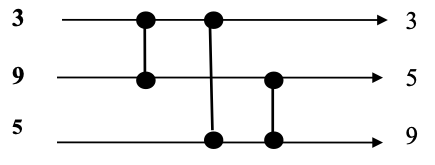
\includegraphics[scale=0.4]{images/sorting_network.png}
    \caption{Rete per l’ordinamento di $3$ interi}
\end{figure}

\begin{definizione}
    Le istruzioni di confronto per i confrontatori o comparatori
    $$\text{if}\;A[i]<A[j]\;\text{then SWAP}\;(A[i], A[j])$$
    $$\text{if}\;A[i]>A[j]\;\text{then SWAP}\;(A[i], A[j])$$
\end{definizione}

Insieme di confrontatori tali per cui passandogli un input mi torna un output ordinato. Formalmente definiamo una rete di confrontatori con
$$R(x_1, \dots , x_n) = (y_1, \dots , y_n)$$
Si dice che R è una sorting network sse 
$$\forall (x_1, \dots , x_n) \in N^2 \; vale\; R \; con\; y_1 < y_2 < \dots < y_n$$

Queste reti si chiamano anche reti di ordinamento \textit{TEST/SWAP OBLIVIOUS}, deriva dal fatto che i confronti che vengono eseguiti non dipendono dall'input, sono state fissate a priori, vengono effettuati qualunque sia l'input. Come faccio a sapere se R è una sorting network?

\paragraph{Principio 0-1 (Knut 1972)}
Uno strumento che grandemente semplifica le dimostrazioni di correttezza delle procedure di ordinamento su reti. Valuto la sorting network solo su valori binari

\begin{definizione}
    Se una rete di ordinamento R lavora correttamente su vettori con componenti in ${0,1}$, allora lavora correttamente per qualsiasi vettore di interi
\end{definizione}

\paragraph{Asserzione di Knut}
$$\exists \; x \in N^n \;t.c\; R(x)\;non\;e'\;ordinato$$
Esiste un $x$ che non viene ordinato da $R$.
$$\exists \; x \in \{0,1\}^n \;t.c\; R(x)\;non\;e'\;ordinato$$
Cioè non funziona bene nemmeno in binario

\paragraph{Dimostrazione Knut}
All'input prima viene applicata la funzione \textit{f}, in uscita viene applicata \textit{R} che è la mia rete di confrontatori. Il risultato non cambia se shiftiamo f su R, cioè se invertiamo (prima R poi f). \uline{Affinchè questo sia vero bisogna assumere che la funzione \textit{f} sia monotona crescente}. \uline{f-shift su R vale per ogni f monotona crescente}

Se esiste un $x$ tale che $R(x)$ non lo ordina deve valere che $R(x)$ restituisce un vettore $y$ dato dalle componenti $y_1, \dots, y_n$ tale che due elementi non sono ordinati. Deve esistere un $y_k$ che precede un $y_s$ che è più grande.

$$\exists\; x \in N^n \;t.c.\; R(x) = (y_1, \dots, y_k, y_s, \dots, y_n )\; con\; y_k > y_s$$

Definiamo una funzione G monotona crescente $N \rightarrow {0,1}$
\begin{equation}
    g(x) = 
        \begin{cases}
            1 & \text{se $x \geq y_k$}\\
            0 & \text{altrimenti}
        \end{cases}
\end{equation}

Calcolo R su un vettore binario 
$$R(g(x_1), \dots , g(x_n))$$
Posso applicare la regola dello shift (g-shift), prima applico R poi g, otteniamo in ouput un vettore binario e dobbiamo vedere se è stato ordinato oppure no
$$= (g(x_1), \dots , g(y_k), \dots, g(y_s), \dots , g(y_n))$$

Non è ordinato perchè $y_k > y_s$. La rete sbagliava su $x$, sbaglia anche sul binario.

\begin{osservazione}
Come faccio a sapere se R è una sorting network? Se voglio scoprire se una rete è una sorting network mi basta valutare R solo su input binari.
\end{osservazione}

\subsection{Array lineare}
Sono un'architettura a memoria distribuita. I processori sono connessi uno in fila all'altro su una riga. Ogni processore è collegato al processore precedente e al suo successivo

\paragraph{Parametri di rete}
$\gamma = 2\;, \;\delta = n-1\; ,\; \beta = 1$. Un $\gamma$ così è il più basso che possiamo avere, altrimenti non ci sarebbero i collegamenti. $\delta$ rappresenta la distanza tra i processori più ”lontani” $P_1$ e $P_n$

Nelle P-RAM il tempo è esattamente il tempo dei conti, mentre in questo caso c'è anche il tempo di comunicazione, che non è costante, perciò non sarà possibile ottenere tempi logaritmici.

\subsubsection{Shuffle}
Prende un array lo divide a metà e intercala la prima metà con la seconda metà facendo in prima posizione il primo elemento della prima metà, in seconda posizione il primo elemento della seconda metà poi di nuovo il primo elemento etc$\dots$.   \uline{Mischia intercalando uno della prima metà con uno della seconda metà}

\paragraph{Primitiva shuffle}
Servirà anche sull'ordinamento per altre architetture parallele come Mesh, \uline{swap contiguo}

$$SWAP (k, k+1)$$

Abbiamo due processori consecutivi $P_k$ e $P_{k+1}$ collegati direttamente perchè consecutivi. Il primo ha il dato $A[k]$, il secondo $A[k+1]$. Si richiede di swappare i contenuti. Si utilizzano le istruzioni \uline{send} e \uline{receive}.

In un passo (un giro di clock) fanno le send, all'istante dopo fanno due receive per leggere il dato che gli è stato spedito. \uline{Il numero di passi per questa primitiva è costante ($3$ passi)}. E' costante perchè i processori sono collegati tra di loro

\paragraph{Shuffle}.\\
Input: $A[1]\;A[2]\dots A[s]\;A[s+1]\dots A[2s]$\\
Output: $A[1]\;A[s+1]\;A[2]\;A[s+2]\dots A[s]\;A[2s]$

\uline{In input abbiamo un vettore di lunghezza pari}, in output desideriamo una prima metà dell'input innestata dalla seconda metà. Ossia, vogliamo in output che le due metà siano mischiate.

Sostanzialmente alterniamo i nostri elementi in questo modo: un elemento della prima metà, un elemento della seconda metà.

Su un array lineare di n elementi, lo SHUFFLE di $(a[1], a[2], a[3], \dots, a[2s])$ può essere ottenuto in tempo $O(s)$ da un procedura SHUFFLE con scambi a “triangolo”

\begin{figure}[h]
    \centering
    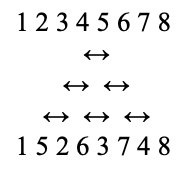
\includegraphics[scale=0.40]{images/shuffle.png}
\end{figure}

\paragraph{Numero di processori}
processori = $2(s-1)$ perchè il primo e l'ultimo elemento non vengono mai scambiati, perciò si può evitare di assegnare un processore

\paragraph{Tempo}
Numero di passi $3$. Tempo parallelo $3(s-1)$, si conta la diagonale sul grafico e risultano essere la metà del nostro input

\paragraph{Efficienza}
Sopra c'è il costo dello shuffle sequenziale senza supporre di avere una memoria aggiuntiva. Sotto numero di processori per tempo parallelo. Il risultato è un algoritmo ottimale.
$$E \approx \frac{s^2}{s\;*\;s} = C$$

\subsubsection{Max}
Visto che i dati sono distribuiti nelle memorie private dei nostri processori ci sarà la richiesta di spedizione del dato. $P_i$ deve spedire il proprio dato $A[i]$ al processore $j$.

\paragraph{Primitiva Max}
$SEND(i,j)$ dove $i$ è il sender, $j$ il receiver. Entra in gioco la distanza tra i due processori


\paragraph{Max}.\\
Input: $A[1]\;A[2]\dots A[n]$\\
Ouput: $contenuto(P_n) = max\{\;A[i]\;|\;1 \leq i \leq n\;\}$

\uline{Mettiamo il risultato nel processore che ha indice più alto}. Il tempo per MAX su array lineari è limitato inferiormente da \textit{n}. Anche qui possiamo applicare l'idea di Wyllie

\begin{enumerate}
    \item Si considera l'algoritmo per SOMMATORIA delle P-RAM
    \item Riduzione dei processori per abbassare $\Omega(n)$ su array ad $n$ processori, che può essere confrontato con il tempo degli algoritmi sequenziali per risolvere lo stesso problema
\end{enumerate}

Stesso ragionamento che si fa per sommatoria, al j-esimo passo si confrontano i numeri a distanza $2^{j-1}$

\begin{itemize}
    \item Confronto con numeri a distanza $2^j-1$
    \item Selezione del max
    \item Memorizzo nel processore di indice $2^j\;*\;t$
\end{itemize}

\paragraph{Codice}
\begin{minted}
[
frame=lines,
framesep=2mm,
baselinestretch=1.2,
bgcolor=white,
fontsize=\footnotesize,
linenos
]{python}
for j in range(1, logn + 1):
    for t in range(1, n // (2**j) + 1):
        k = 2**j * t - 2**(j-1)
        SEND(k, k + 2**(j-1))

    for t in range(1, n // (n // (2**j)) + 1):
        k = 2**j * t
        if A[k] < A[k - 2**(j-1)]:
            A[k] = A[k - 2**(j-1)]
\end{minted}

\paragraph{Tempo}
Calcoliamo il tempo per la \textit{send} e il tempo per il \textit{compare} poi moltiplichiamo per $\log n$. La prima è $2$ volte la distanza tra i processori quindi $2*2^{j-1}$. La seconda fase richiede un confronto ed un eventuale assegnamento, quindi costa $2$

$$Totale = \sum_{j=1}^{\log n} 2\; 2^{j-1} + \sum_{j=1}^{\log n} 2 = \sum_{j=1}^{\log n} 2^j + 2\log n = 2^{\log n+1}-1-1 + 2 \log n = 2n - 2 + 2 \log n = O(n)$$

\paragraph{Processori} Il numero dei processori è tanto quanto la lunghezza dell'input $n$

\paragraph{Efficienza} $E \rightarrow 0$, non va bene

\paragraph{Nuovo algoritmo}
\begin{osservazione}
    Se riduciamo i processori da $n$ a $p$, ogni processore deve prendersi $\frac{n}{p}$ elementi. In questo modo operiamo sul parametro $\delta$ cioè la distanza massima tra i processori, perchè da $n$ sono passato ad un array di $p$ elementi e questo valore viene ridotto
\end{osservazione}
\begin{itemize}
    \item Un processore seleziona il max sequenzialmente tra i suoi $\frac{n}{p}$ processori
    \item Si esegue il codice per MAX su $p$ processori (fase di spedizione dei massimi)
\end{itemize}

\paragraph{Prestazioni} Processori: P; Tempo parallelo: $O(\frac{n}{p}) + O(p)$

\paragraph{Efficienza}
Al numeratore abbiamo $n$ (calcolo del massimo sequenzialmente, tempo lineare) al denominatore abbiamo $P\;*\;tempo\;parallelo$ $P(O\frac{n}{p} + O(p)) = O(n) + O(p^2)$

Per avere $E \rightarrow C \neq 0$ scelgo $p^2 = n$. Scelgo $p$ in modo tale che il quadrato mi da n, cioè $p = \sqrt{n}$

Di conseguenza MAX è risolto efficientemente su array lineari con $P=\sqrt{n}$ e 
$$T=O(\frac{n}{\sqrt{n}} + O(\sqrt{n})) = O(\sqrt{n})$$


\subsubsection{Ordinamento}
In questo caso lo SWAP può essere anche su processori non contigui, \uline{generalizziamo l'operazione di SWAP}.

\paragraph{Primitiva}
MINMAX $(K, K+1)$. Abbiamo due processori $P_k$ e $P_{k+1}$, il primo deve contenere il minimo valore, il secondo deve contenere il massimo. \uline{Questo problema è del tutto simile allo SWAP, ma non sempre avviene lo scambio di dati}. \uline{Al posto di esserci l'assegnamento sicuro, c'è un assegnamento condizionato}. C'è un if e poi un eventuale assegnamento, il numero di passi paralleli per risolverlo è un passo in più, quindi $4$

\uline{Minmax è la primitiva che realizza il confrontatore nelle sorting network}

\paragraph{Ordinamento}
Abbiamo $n$ dati, ognuno viene lasciato ad un processore. Come output desideriamo leggere il risultato sui nostri processori seguendo l'indice dei processori.

\paragraph{ODD/EVEN sorting network} Un algoritmo \textit{test/swap oblivious} descritto da una sorting network

L'ordinamento odd-even è un algoritmo di ordinamento parallelo che viene utilizzato per ordinare una serie di elementi in modo efficiente su più processori o su una rete di calcolatori. \uline{L'algoritmo funziona confrontando elementi in posizioni dispari con elementi in posizioni pari e scambiandoli se sono in ordine sbagliato}. Ciò viene ripetuto per ogni coppia di elementi consecutivi nella serie, fino a quando l'intera serie non è stata ordinata

\begin{figure}[h]
    \centering
    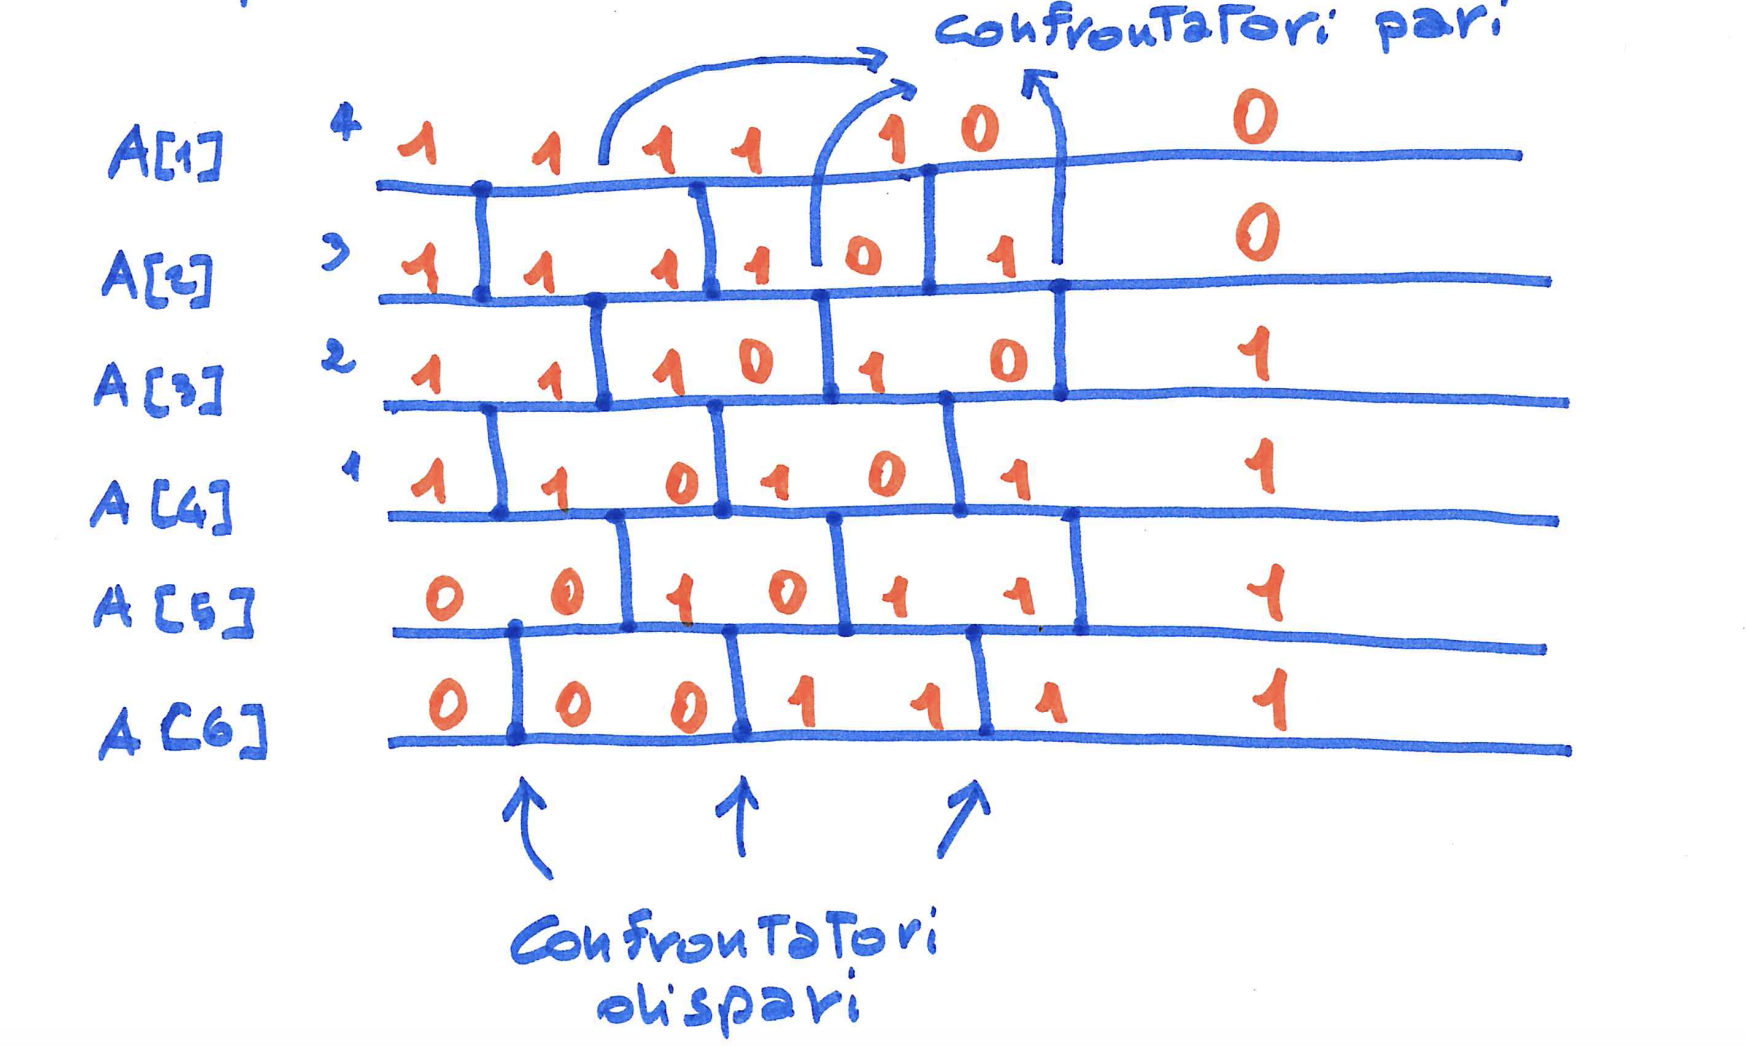
\includegraphics[scale=0.4]{images/odd_even.png}
    \caption{Esempio con 6 elementi da ordinare}
\end{figure}

Al primo passo non viene mai confrontato un $1$ con uno $0$. Il primo passo non scambia nessun elemento dell'input. Esempio: il secondo $0$ inizia a muoversi dal terzo passo

\uline{Per la correttezza di ODD/EVEN usiamo il principio $0-1$ (Knuth)}. Se questa rete mi ordina tutti i numeri binari, allora è una rete che è corretta anche sui numeri naturali. 

$$\{0,1\}^n \rightarrow\;odd/even\; \rightarrow 0^j1^e\;con\;j+e=n$$

\paragraph{Dimostrazione}
Ci vogliono $n$ round, che sono necessari si vede dall'esempio, ma che sono sufficienti lo dobbiamo dimostrare

Partiamo dall'esempio, abbiamo $4$ volte $1$ e $2$ volte $0$, quindi $e=4\;;\;j=2$

\begin{osservazione}
    Nel nostro caso ogni $1$ deve scendere di $n - e = j = \# 0$ posizioni. Cioè ogni $1$ deve scendere di almeno $2$ posizioni.
\end{osservazione}

Si possono studiare gli $1$ dal basso più il ritardo. Il massimo ritardo che si può avere è il numero di $1$ dell'input
\begin{itemize}
    \item La regola è che l'i-esimo dal basso impiega $n - e + i$ passi
    \item In generale è un \textit{al più} $n - e + i$ passi
    \item Dato che $i \leq e$ si ottiene $n - e + e = n$ passi, al più $n$ passi $\implies n$ passi di ODD/EVEN sono necessari e sufficienti
\end{itemize}

\paragraph{Implementazione con codice}
\begin{itemize}
    \item Sequenziale $T(n) = O(n^2)$
    \item Parallelo Haberman $'72$\\
    $n$ passi paralleli o round di comparatori implementati con MINMAX
    \begin{lstlisting}
        for i = 1 to n
            for k in {2t - (i%2) | 1 <= t <= n/2} par do
                MINMAX(k, k+1)
    \end{lstlisting}

    Il primo round fa lavorare con MINMAX quelli con indice dispari
\end{itemize}

\paragraph{Tempo}
For esterno mi dice quanti round ci sono, n colonne di comparatori. Il MINMAX che viene eseguito in parallelo dal for par do richiede $4$ istruzioni (come lo SWAP ma con il confronto), perciò

$$n * 4 = O(n)$$

dove $n$ è il numero di round e $4$ è il min-max in parallelo

\paragraph{Efficienza}
$$\frac{n\;\log n}{n\;n} \rightarrow 0 $$

%Riduzione dei processori
\begin{comment}
    \paragraph{Riduzione dei processori}
Primo step: ogni processore si prende $\frac{n}{p}$ dati e li ordina
\end{comment}

\paragraph{Primitiva MERGE-SPLIT}
La primitiva MERGE-SPLIT avviene tra due processori contigui
\begin{itemize}
    \item Il processore di sinistra spedisce $\frac{n}{p}$ dati ordinati al processore di destra. Questo ha tempo $O(\frac{n}{p})$
    \item (MERGE) Il processore di destra riceve e fonde i nuovi $\frac{n}{p}$ con i suoi $\frac{n}{p}$ dati (ordinati). Questo ha tempo $O(\frac{n}{p})$
    \item (SPLIT) Il processore di destra invia i dati più piccoli $\frac{n}{p}$ al processore di sinistra
\end{itemize}

Come il codice precedente ma al posto di MINMAX c'è il MERGESPLIT. \uline{E' ODD-EVEN dove minmax è sostituito con la primitiva merge-split}. \uline{Ogni singola primitiva merge-split viene ripetuta per P round}

\paragraph{Tempo}
$$\frac{n}{p} \log \frac{n}{p} + p * \frac{n}{p} = O(n)$$
Primo passo che è sequenziale e lo fanno tutti i processori, più p round per merge-split che richiede $\frac{n}{p}$, le $p$ si semplificano

\paragraph{Denominatore di E}
TODO $\dots$

\paragraph{Efficienza}
$$\frac{n \log n}{n \log n} \rightarrow C \neq 0$$

\begin{osservazione}
    Il tempo è rimasto $O(n)$, ciò si spiega in quanto la riduzione dei processori agisce sul diametro e non sull'ampiezza di bisezione, $\beta = 1$
\end{osservazione}


%Mesh
\subsection{Architetture Mesh}
Processori strutturati a forma di quadrato, con delle connessioni sia per riga che per colonna. Un quadrato di processori connessi sia per riga che per colonna. \uline{Array bi-dimensionale, ovvero una griglia di processori}. I processori sono messi in un quadrato di lato $\sqrt{n}$

\begin{figure}[h]
    \centering
    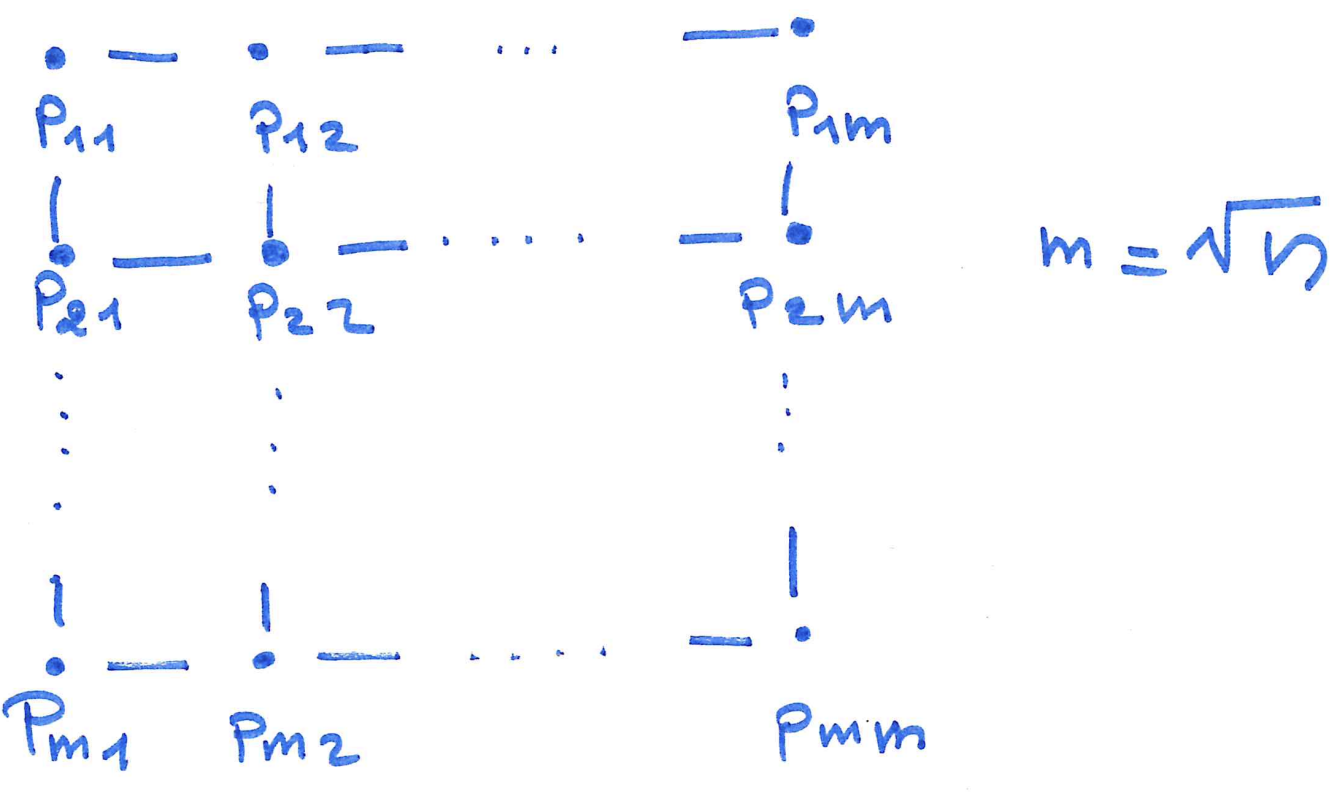
\includegraphics[scale=0.4]{images/architetture_mesh.png}
\end{figure}

\paragraph{Parametri di rete}
\begin{itemize}
    \item $\gamma = 4$ (grado). Il massimo numero di archi incidenti su un nodo, due rivolti sulla riga, due sulle colonne
    \item $\delta = 2\sqrt{n-1}$ (diametro), perchè ci sono i link verticali ed orizzontali quindi percorro la diagonale. I processori più “lontani” sono $P_{11}$ e $P_{mm}$ : essi sono collegati da un cammino di $2(m-1)$ passi.
    \item $\beta \approx \sqrt{n} $, posso tagliare a metà della prima colonna con una riga orizzontale oppure in verticale
\end{itemize}

\begin{figure}[h]
    \centering
    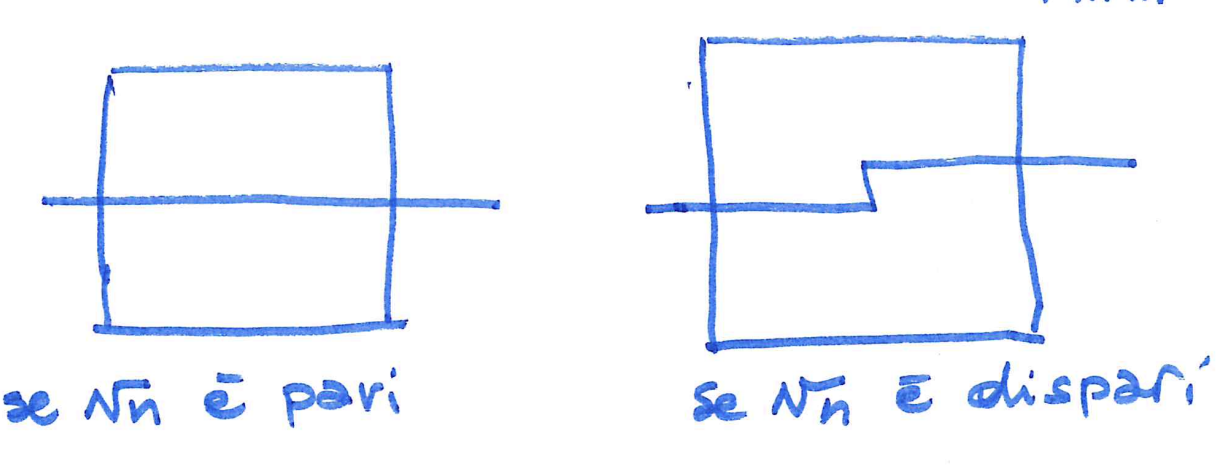
\includegraphics[scale=0.4]{images/architettura_mesh2.png}
\end{figure}

\paragraph{Lower bound}
Visto che il diametro e il $\beta$ sono nell'ordine $\sqrt{n}$ abbiamo questi lower bound
\begin{itemize}
    \item MAX $\Omega(\sqrt{n})$
    \item ORDINAMENTO $\Omega(\sqrt{n})$
\end{itemize}

\subsubsection{Max}
\paragraph{Serpente}
Potremmo vedere nella nostra architettura mesh un "serpente" di processori. Posso costruire un percorso a serpente fino ad arrivare all'ultima riga, ottenendo così un array lineare. A questo punto prendo l'algoritmo del massimo su array lineare e lo eseguo

\uline{Usiamo la Mesh come array lineare}. In questo serpente ci sono $n$ processori e la distanza tra due processori più lontani risulta essere $n$ e quindi la soluzione sul serpente non può richiedere meno di $n$ passi paralleli, e non va bene visto il lower bound.

Definisce un ordine con cui leggere i dati nella mesh, i primi $m$ valori vengono dati sulla prima riga, nella seconda riga si va da destra verso sinistra. Anche l'output dovrà essere letto in questo modo

Se vogliamo sfruttare questo come un array lineare non otteniamo dei risultati migliori dell'array lineare 

\paragraph{Algoritmo RIGHE-COLONNA per MAX}
\uline{Ogni riga dell'array e l'ultima colonna sono viste come array lineare di $\sqrt{n}$ processori separati}. Posso calcolare il massimo su ogni riga, sposto l'elemento massimo di ogni riga nell'ultima posizione della riga. Dopodichè nell'ultima colonna ho tutti gli elementi massimi e posso calcolare il massimo degli elementi massimi vedendo questa colonna come un array lineare che verrà posizionato in $P_{mm}$.

\paragraph{Codice}
\begin{minted}
[
frame=lines,
framesep=2mm,
baselinestretch=1.2,
bgcolor=white,
fontsize=\footnotesize,
linenos
]{python}
for i in range(1, int(sqrt(n)) + 1):
    MAX(pi, pi2, ..., pim)
    +
    MAX(p1m, p2m, ..., pmm)
\end{minted}
Il primo MAX fa il massimo di un'array lineare di ogni riga $i$ che va da $1$ a $\sqrt{n}$. Richiede come tempo/numero di passi pari alla dimensione dell'array lineare ($\sqrt{n}$)

Il secondo MAX è il massimo dell'ultima colonna. Entrambi i max hanno tempo $\sqrt{n}$, quindi $O(\sqrt{n})$, come il lower bound. I processori coinvolti sono quelli con indice pari ad $m$, anche questi formano un array lineare, l'ultima colonna.

\paragraph{Efficienza}
$$E = \frac{n}{n\;\sqrt{n}} \rightarrow 0$$
La cosa non funziona bene, l'idea è quella di operare una \uline{riduzione dei processori} per ottenere un'efficienza migliore

\paragraph{Operiamo una riduzione dei processori}
Il numero dei processori va da $n$ a $p$. Ogni processore si prenderà un gruppetto $\frac{n}{p}$ elementi su cui calcolare il massimo

\begin{itemize}
    \item Ogni processore calcola il MAX tra $\frac{n}{p}$ dati che richiede un tempo sequenziale di $O(\frac{n}{p})$
    \item Si attiva l'algoritmo RIGHE-COLONNE però su una griglia che non è più $\sqrt{n}\;*\;\sqrt{n}$ ma è diventata $\sqrt{p}\;*\;\sqrt{p}$. La nostra gliglia ha lato $\sqrt{p}$, quindi il tempo è $O(\sqrt{p})$, sommando la prima fase $O(\sqrt{p}) + \frac{n}{p} + \sqrt{p}$
\end{itemize}

Voglio un'efficienza che sia $\frac{n}{n}$, perciò scelgio $p^{\frac{3}{2}} = n \implies p = \sqrt[3]{n^2} = n^{\frac{2}{3}}$

\paragraph{Tempo}
Prima fase costa $\sqrt[3]{n}$, seconda fase $\sqrt[3]{n}$, in totale avrò $O(\sqrt[3]{n})$

\subsubsection{Ordinamento}
\textbf{Input}: $n$ numeri distribuiti uno per processore. Se l'indice della riga è dispari vengono distribuiti da sinistra verso destra, se pari da destra verso sinistra (a serpente)\\
\textbf{Output}: $n$ numeri ordinati secondo il percorso a \textit{serpente}. Ci aspettiamo un output ordinato crescente

Presentiamo qui un algoritmo che risolve su mesh il problema ORDINAMENTO in tempo ottimo $O(n)$; \uline{per semplicità, prenderemo in considerazione mesh $mxm$ dove m è potenza di $2$}

\paragraph{Ordinamento LS3}
Il nome deriva dai cognomi degli inventori degli anni $'80$. L'algoritmo è \uline{ricorsivo}, cioè richiama se stesso su istanze più piccole, applicando la tecnica \uline{dividi-et-impera}.

Chiamiamo $M$ l'intero quadrato dei processori

Esattamente come il \textit{Merge-sort}, ma quest'ultimo non prendeva i dati dalla struttura di un quadrato ma da una riga.

\paragraph{Dividi}
Abbiamo una struttura quadrata, va rispettata questa forma e si divide il quadrato in $4$ sotto-quadrati di lato la metà. Se il lato è $n$, dividiamo l'input in quadrati di dimensione $\frac{n}{2}$


\paragraph{Ordina}
Con le chiamate ricorsive si riesce ad ordinare ogni metà. Leggiamo l'input ordinato a \textit{serpente}


\paragraph{Fondi}
Una volta che arrivano quattro matrici ordinate $M_1, M_2, M_3, M_4$ l'algoritmo fonde restituendo la matrice M totalmente ordinata. Gli elementi si leggono a \textit{serpente}

\paragraph{Codice parallelo}.
\begin{minted}
[
frame=lines,
framesep=2mm,
baselinestretch=1.2,
bgcolor=white,
fontsize=\footnotesize,
linenos
]{python}
procedure LS3sort(M):
    if len(M) == 1:
        return M
    else:
        M1 = LS3sort(M1)
        M2 = LS3sort(M2)
        M3 = LS3sort(M3)
        M4 = LS3sort(M4)
        return LS3merge(M1, M2, M3, M4)
\end{minted}

Le chiamate \textit{LS3sort} sono in parallelo

\paragraph{LS3merge}
Si fanno due operazioni
\begin{itemize}
    \item SHUFFLE\\
    In LS3merge si fa shuffle di ogni riga. \uline{Prende tutte le matrici e la considera un'unica matrice}, facendo shuffle sulle sue righe. Alternando un elemento della prima metà con un elemento della seconda metà. Si costruisce M in questo modo. \uline{Inframezzare ed alternare un elemento della prima metà con un elemento della seconda metà}
    
    \item ODD/EVEN\\
    Ordinamento odd/even su due colonne adiacenti. Vuole vedere queste due colonne come un array lineare, anche questa volta le connessioni sono fatte a serpente. 
\end{itemize}

\paragraph{LS3merge: codice}.
\begin{minted}
[
frame=lines,
framesep=2mm,
baselinestretch=1.2,
bgcolor=white,
fontsize=\footnotesize,
linenos
]{python}
procedure LS3merge(M1, M2, M3, M4):
    for i in range(1, int(sqrt(n)) + 1):
        SHUFFLE(i)

    for i in range(1, int(sqrt(n/2)) + 1):
        ODD_EVEN(2*i - 1, 2*i)

    execute the first 2 * sqrt(n) steps of ODD_EVEN
    on the entire mesh (in a snake pattern)
\end{minted}

\paragraph{LS3merge: tempo parallelo}

Tutti e $3$ i passaggi del codice hanno tempo $O(\sqrt{n})$ perciò
$T_{merge}(n) = h\sqrt{n}$

\paragraph{Tempo}
Equazione di ricorrenza
\begin{equation}
    T(n) = 
        \begin{cases}
            1 & \text{se $n=1$}\\
            $T(N/4) + h\sqrt{n} & \text{altrimenti}$
        \end{cases}
\end{equation}

\newpage



